\section{程序的使用测试}

\subsection{测试的意义及方法}

1)  测试的意义:测试的意义去检验程序中的是否存在错误,是否满足文所需要实现的签名及验证的功能。通过输入常规数据和非常规数据观察程序是否满要求。同时对测试所用数据要具有一般性,并对输入数据的有一个相应的输出期望结果,并通过对不同数据的修改观察程序是否运作正常,结果是否与期望结果一致。

2)  测试方法:先对测试用例data.txt进行签名、代理签名、验证签名及验证代理签名等操作,再改变原消息值即data.txt里的文字,再进行验证签名及验证代理签名操作,观察分析得到的结果。

\subsection{测试Elgamal签名方案}

\subsubsection{测试用例}

测试用例:1、大小为128字节的txt文档。

          2、大小为340字节的txt文档。

\subsubsection{测试过程}

1)生成公私钥对

    运行程序,根据主界面,选1,生成Elgamal公私钥对,公钥y,大素数p,本原元g保存在pub.txt;私钥x,大素数p,本原元g保存在pri.txt:

\begin{figure}[H]
\centering
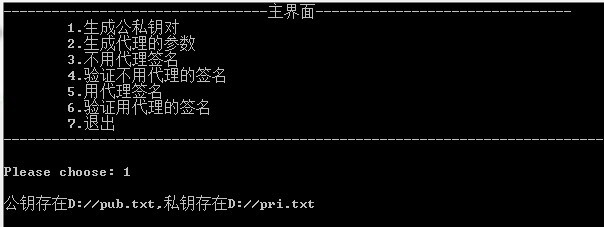
\includegraphics{img/7.jpg}
\caption{生成公私钥}
\end{figure}

Pub.txt文件中,由上至下三个大数依次为:公钥y,大素数p,本原元g

\begin{figure}[H]
\centering
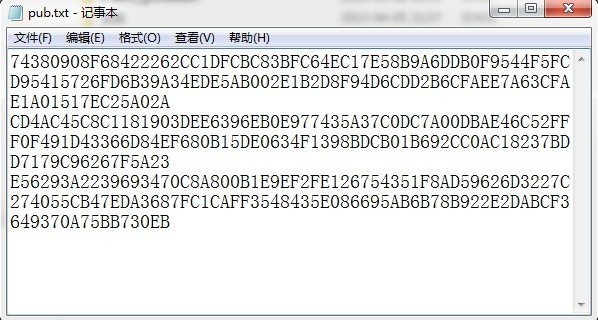
\includegraphics{img/8.jpg}
\caption{pub.txt}
\end{figure}

pri.txt,由上至下三个大数依次为私钥x,大素数p,本原元g:

\begin{figure}[H]
\centering
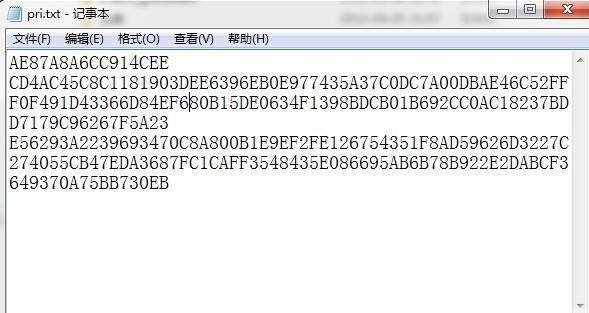
\includegraphics{img/9.jpg}
\caption{pri.txt}
\end{figure}

2)签名与验证签名
   对大小为128字节的data.txt进行签名操作,签名耗时3毫秒:

\begin{figure}[H]
\centering
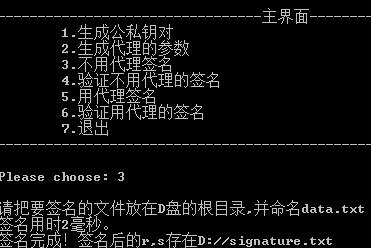
\includegraphics{img/10.jpg}
\caption{对data.txt签名}
\end{figure}

128字节的data.txt内容:

\begin{figure}[H]
\centering
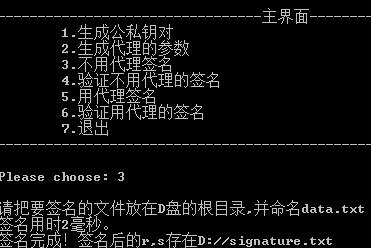
\includegraphics{img/10.jpg}
\caption{data.txt}
\end{figure}

生成的签名(r,s)保存在signature.txt中:

\begin{figure}[H]
\centering
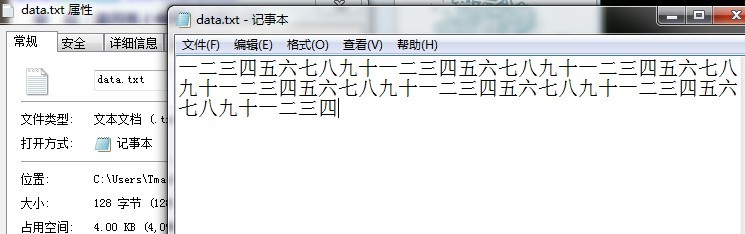
\includegraphics{img/11.jpg}
\caption{生成的签名(r,s)}
\end{figure}

验证签名。此签名是正确的:

\begin{figure}[H]
\centering
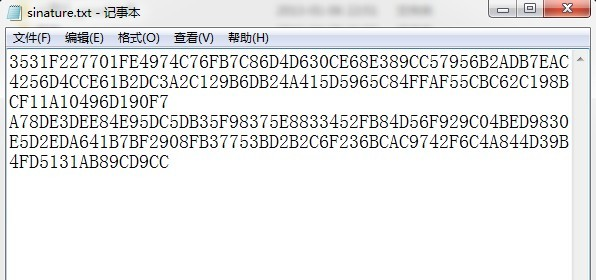
\includegraphics{img/12.jpg}
\caption{验证签名}
\end{figure}

改变data.txt的内容为:

\begin{figure}[H]
\centering
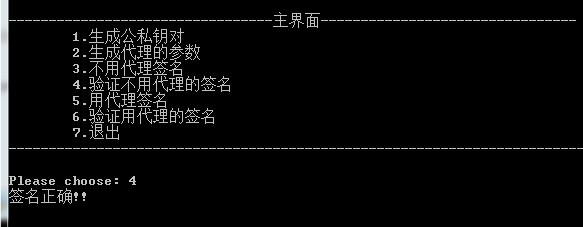
\includegraphics{img/13.jpg}
\caption{原data.txt被修改后}
\end{figure}

然后执行一次验证签名操作结果如下:

\begin{figure}[H]
\centering

\includegraphics{img/14.jpg}
\caption{签名有误}
\end{figure}

对大小为340字节的data.txt进行一组同样的操作

Data.txt

\begin{figure}[H]
\centering
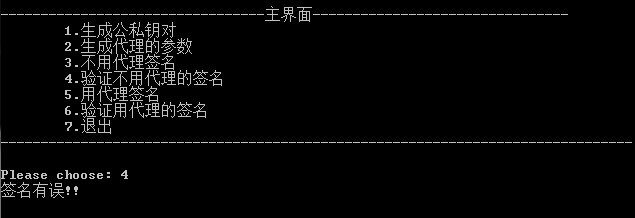
\includegraphics{img/15.jpg}
\caption{data.txt}
\end{figure}

签名

\begin{figure}[H]
\centering
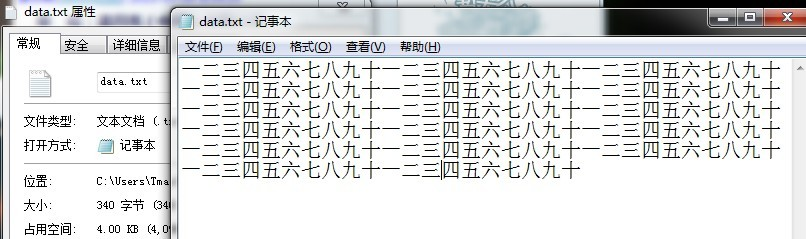
\includegraphics{img/16.jpg}
\caption{签名}
\end{figure}

验证签名

\begin{figure}[H]
\centering
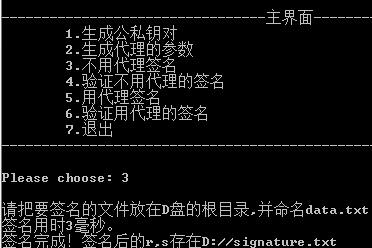
\includegraphics{img/17.jpg}
\caption{验证签名}
\end{figure}

改变data.txt的内容

\begin{figure}[H]
\centering
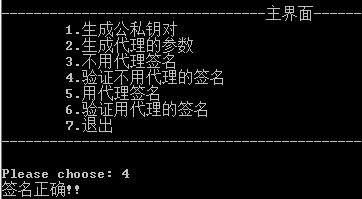
\includegraphics{img/18.jpg}
\caption{data.txt被修改}
\end{figure}

再验证一次签名

\begin{figure}[H]
\centering
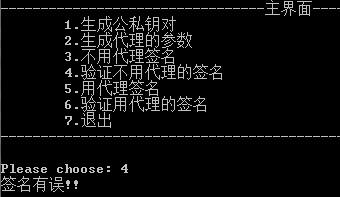
\includegraphics{img/20.jpg}
\caption{原文被改后签名有误}
\end{figure}

\subsubsection{结果分析}

如上面步骤所示,对不同长度data.txt进行签名和对data.txt验证签名得到了与预期相符的结果;而后面原文被窜改,依然对同样的签名进行验证签名,得到的结果是签名有误!与预期结果相符。

\subsection{基于Elgamal算法的代理签名方案的实现}

\subsubsection{测试用例}

测试用例:1、大小为128字节的txt文档。

          2、大小为340字节的txt文档。

\subsubsection{测试过程}

1)  进入系统主界面,选1生成公私钥对,在有了pub.txt和pri.txt数据的情况下,生成代理签名的参数。私密共享给代理签名者的参数d,K,p,g存入proxy\_pri.txt,公布出去的原始签名者的公钥y,代理参数K,p与g存入proxy\_pub.txt中:

\begin{figure}[H]
\centering
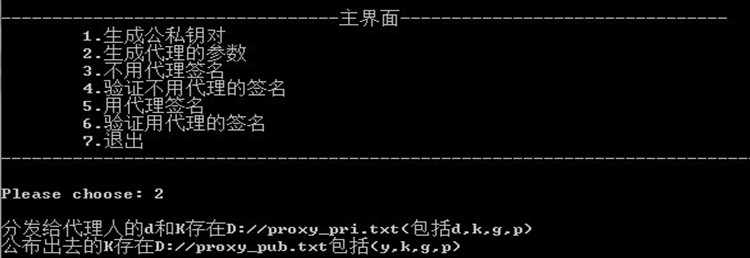
\includegraphics{img/21.jpg}
\caption{proxykeys}
\end{figure}

Proxy\_pri.txt中,由上至下分别为x,K,p,g:

\begin{figure}[H]
\centering
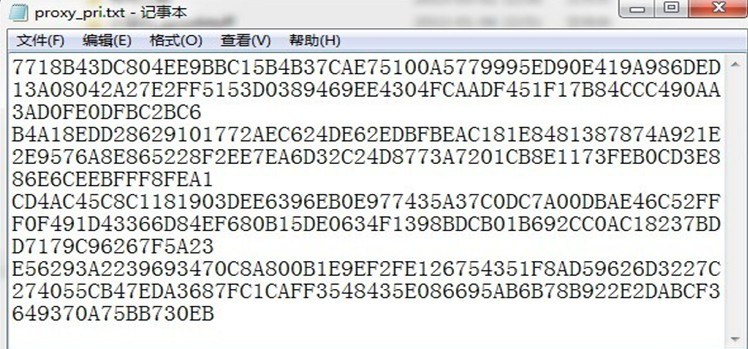
\includegraphics{img/22.jpg}
\caption{proxy\_pri.txt}
\end{figure}

Proxy\_pub.txt中,由上至下分别为原始签名者的公钥y,代理参数K,p与g:

\begin{figure}[H]
\centering
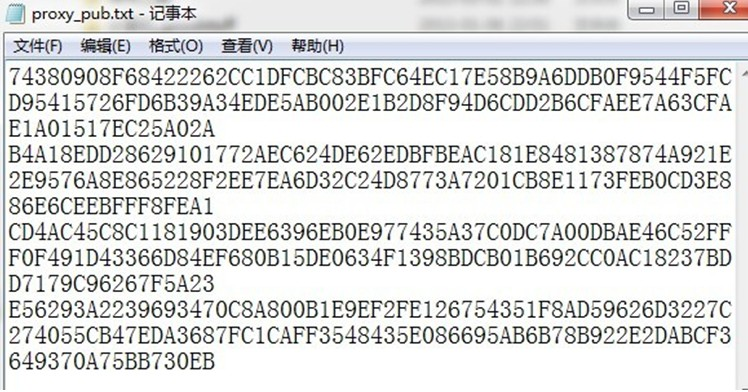
\includegraphics{img/23.jpg}
\caption{proxy\_pub.txt}
\end{figure}

2)  代理签名与验证代理签名

对大小为128字节的data.txt使用代理密钥进行数字签名操作,此步骤包涵对代理参数的检验,即每一次签名前都会检验代理参数是否有效。

\begin{figure}[H]
\centering
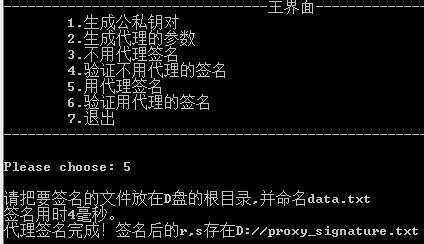
\includegraphics{img/24.jpg}
\caption{proxy-signature}
\end{figure}

签名耗时4毫秒,得到的代理签名(R,s):

\begin{figure}[H]
\centering
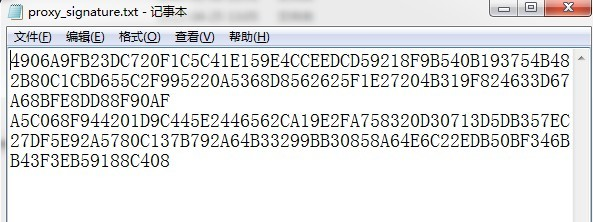
\includegraphics{img/25.jpg}
\caption{proxy-signature.txt}
\end{figure}

验证代理签名,签名正确:

\begin{figure}[H]
\centering
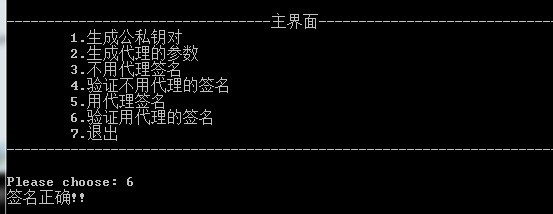
\includegraphics{img/26.jpg}
\caption{签名正确}
\end{figure}

修改data.txt内容为:

\begin{figure}[H]
\centering
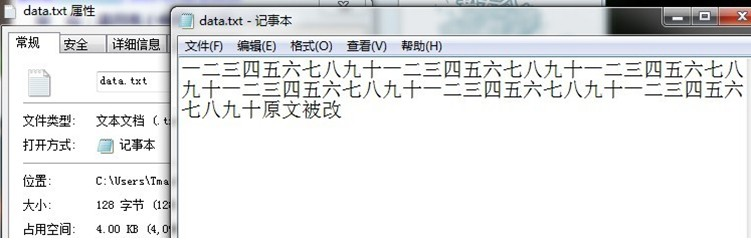
\includegraphics{img/28.jpg}
\caption{修改后的data.txt}
\end{figure}

再验证Elgamal代理签名:

\begin{figure}[H]
\centering
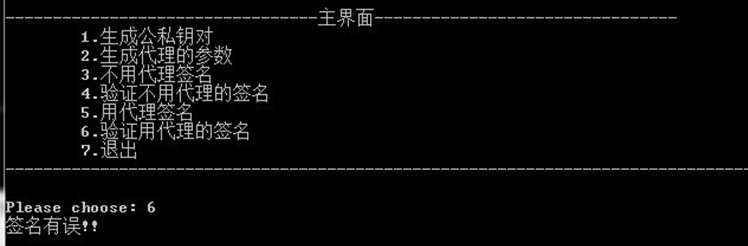
\includegraphics{img/29.jpg}
\caption{原文被改,代理签名有误}
\end{figure}

对大小为340字节的data.txt文档进行一组同上的代理签名与代理签名验证的操作:

data.txt:

\begin{figure}[H]
\centering
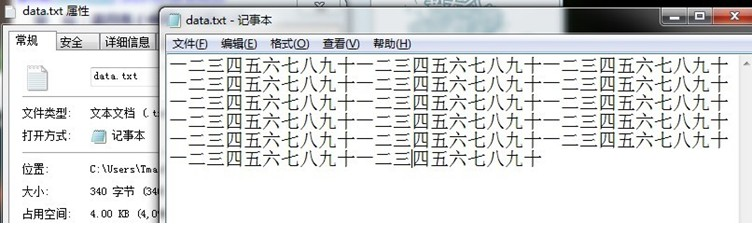
\includegraphics{img/30.jpg}
\caption{340字节的data.txt}
\end{figure}

进行代理签名:

\begin{figure}[H]
\centering
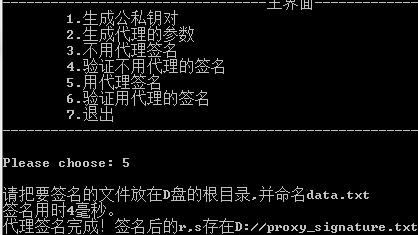
\includegraphics{img/31.jpg}
\caption{代理签名}
\end{figure}

验证代理签名

\begin{figure}[H]
\centering
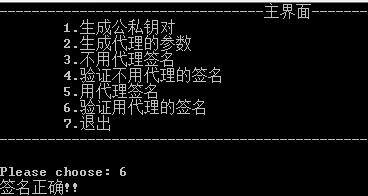
\includegraphics{img/32.jpg}
\caption{验证代理签名,正确!}
\end{figure}

修改data.txt为:

\begin{figure}[H]
\centering
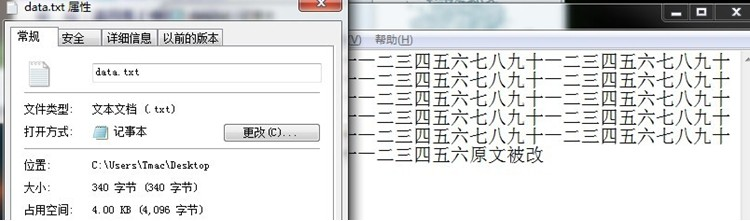
\includegraphics{img/33.jpg}
\caption{修改后的data.txt}
\end{figure}

再验证一次代理签名

\begin{figure}[H]
\centering
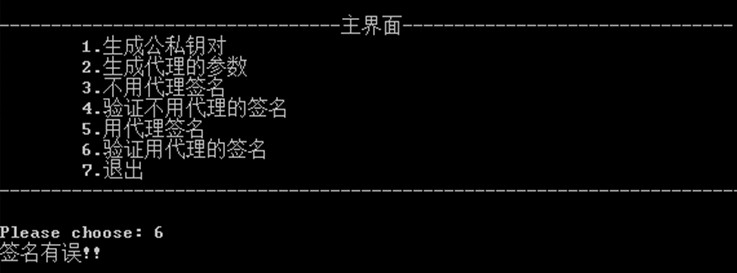
\includegraphics{img/34.jpg}
\caption{原文被改,代理签名验证有误}
\end{figure}

\subsubsection{结果分析}

如上面步骤所示,对不同大小的data.txt进行签名和之后对data\cite{Designated}.txt验证签名都得到了预期的结果,与预期结果相符;而后面原文被窜改,依然对同样的签名进行验证代理签名操作,得到的结果是签名有误!与预期结果相符\cite{计算机密码学及其应用}。